The \emph{blur} effect is one type of degradation that consists of global or local information loss in the image. There are three basic types of blur, generated by different processes: \emph{defocus blur}, \emph{motion blur} and \emph{Gaussian blur}. As explained in \autoref{sec:point_spread_function_and_image_formation_model}, the image formation process is subject to some constraints that limit its quality, such as the presence of noise or the convolution of the formed image with a point spread function. Such convolution results in defocus blur. 

The defocus blur is caused by the incidence of light within an aperture with significant dimensions, where the source of light is not properly placed in accordance to the focal plane; it is related to the variables of the optical system such as depth of focus, aperture, depth of field, aberrations and so on \cite{joshi2014defocus}. According to \citeonline{smith2007modern}, every optical system exhibits blur properties, in higher or lower proportions, due to the depth of focus and its adjustment. Therefore, blurring is unavoidable to a certain extent, hence every imaging device possesses a PSF due to its optics. The PSF is also named \emph{blur kernel}.

The motion blur occurs due to the relative motion between the camera and the scene, e.g. living cells in microscopy, during the acquisition; even though it is considered to be a degradation process, it may be used for aesthetic purposes, such as emphasizing the dynamic nature of a scene, obtaining motion information about the object or creating realistic images which are pleasing to the eye \cite{nayar2004motion}. Motion blur is usually an undesirable effect when it comes to fields such as microscopy, remote sensing or medical imaging, since it compromises analyses, pattern recognition tasks, predictions and several other applications.

The Gaussian blur is a general model of degradation and employs a particular kernel in order to smooth images. A convolution with such kernel promotes a Gaussian average among each region, and is usually employed in photography for styling effects or in edge detection (this application will be explained further in this work). Its kernel \cite{nixon2019feature} is given by

\begin{equation}
\label{eqn:gaussian_blur}
k(x,y) = e^{-
            \left( 
                \frac{x^{2} + y^{2}}{2 \sigma^{2}}
            \right)
            },
\end{equation}

\noindent where $\sigma^{2}$ is the variance of the Gaussian function. \autoref{fig:defocus_motion_blur} shows an example of large scale defocus and motion blur.

\begin{figure}[H]
	\centering
	\caption{\label{fig:defocus_motion_blur}Defocus blur (left) and motion blur (right) in large scales.}
	\begin{center}
	    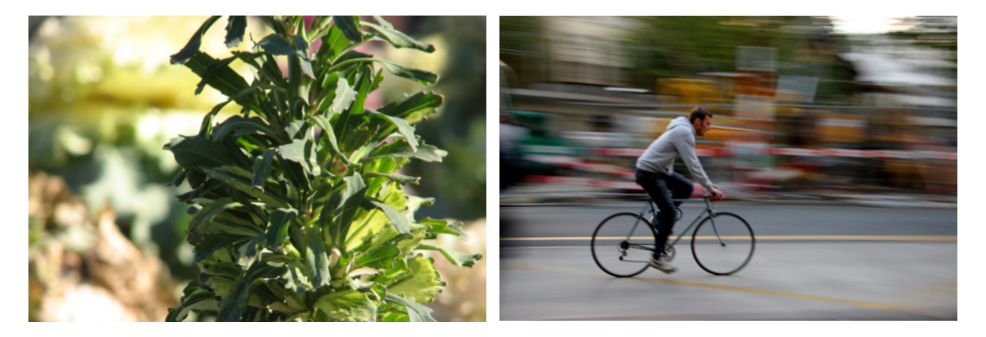
\includegraphics[scale=0.4]{images/fig7.png}
	\end{center}
	\centering
    \fadaptada{su2011blurred}
\end{figure}

Finally, another useful way to mathematically describe the point spread function is through the Dirac Delta. It consists of a generalized function that represents an impulse, i.e. an infinitely high value within an infinitely small period of time \cite{bracewell2000fourier}. \autoref{fig:psf} shows an arbitrary example of a punctual source of light and its image, which suffers the spreading effect.

\begin{figure}[H]
	\centering
	\caption{\label{fig:psf} Magnified image of a light impulse (left) and its impulse response function, the PSF (right).}
	\begin{center}
	    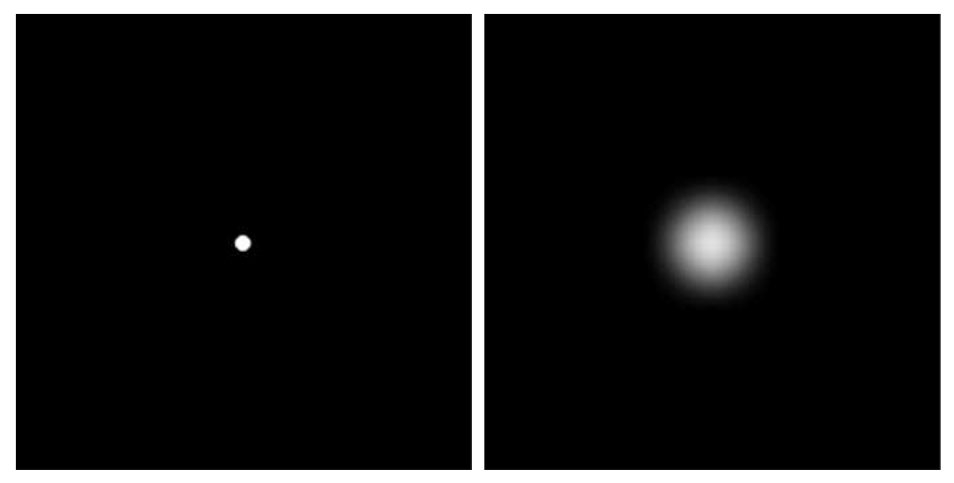
\includegraphics[scale=0.4]{images/fig8.png}
	\end{center}
	\centering
    \fadaptada{gonzalez2008digital}
\end{figure}

Namely, it is a function $\delta(x)$ that is zero-valued for any $x \neq 0$ and is infinity-valued for $x = 0$. This property can be combined with any smooth function $f\colon \mathbb{R}^{n} \to \mathbb{R}^{n}$.
The continuous Dirac Delta may be written, as stated by \citeonline{weisstein2020delta}, as

\begin{align}
\label{eqn:dirac_delta_function}
\delta^{2}(x,y)= 
\begin{cases}
    \infty, & \text{if } x^{2} + y^{2} =0\\
    0, & \text{if } x^{2} + y^{2} \neq 0
\end{cases},
&&
\int_{-\infty}^{\infty}
\int_{-\infty}^{\infty}
\delta^{2}(x,y)dxdy = 1.
\end{align}

\noindent The discrete version of the Dirac Delta function consists of an infinite sum instead of the integral. This concept of impulse is the point source of light, concerning images. It provides the blur effect on images, as it promotes the diffusion of the acquired information.